\shorthandoff{<}
\shorthandoff{>}
\begin{figure}[H]
\center
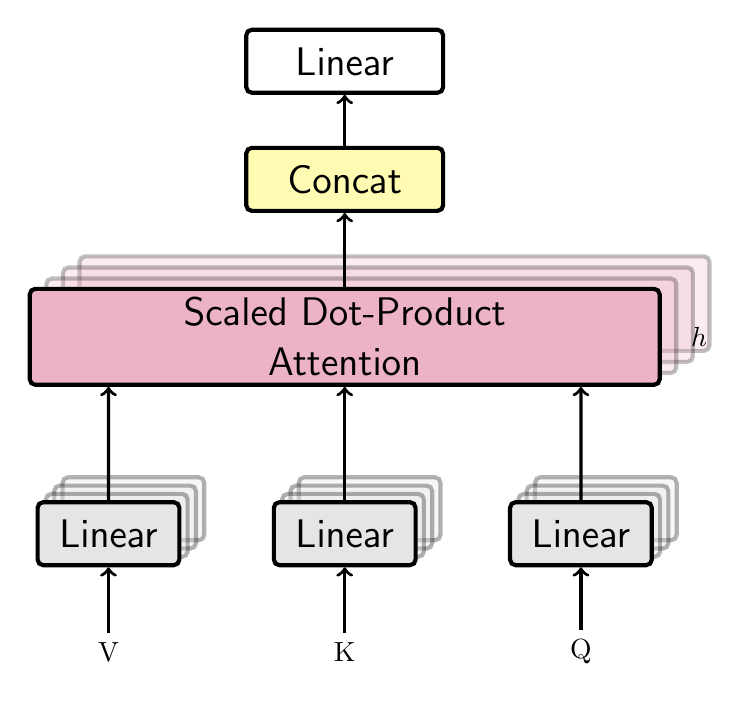
\begin{tikzpicture}[
    box/.style={
        rectangle,
        draw=black,
        line width=1.5pt,
        rounded corners=2pt,
        minimum width=2.5cm,
        minimum height=0.8cm,
        font=\sffamily\Large,
        align=center
    },
    smallbox/.style={
        rectangle,
        draw=black,
        line width=1.5pt,
        rounded corners=2pt,
        minimum width=1.8cm,
        minimum height=0.8cm,
        font=\sffamily\Large,
        align=center
    },
    arrow/.style={->, line width=1.2pt},
]

% Inputs
\node (V) at (-3,0) {V};
\node (K) at (0,0) {K};
\node (Q) at (3,0) {Q};


% === STACKED BACKGROUND (dibujar primero) ===
\foreach \i in {3,2,1} {
    \node[box, fill=purple!30,
        minimum width=8cm, minimum height=1.2cm, xshift=\i*6pt, yshift=\i*4pt, opacity=0.25] (att_box_\i) at (0,4) {};
    \node[smallbox, fill=gray!20,
          xshift=\i*3pt, yshift=\i*3pt, opacity=0.3] at (-3,1.5) {};
    \node[smallbox, fill=gray!20,
          xshift=\i*3pt, yshift=\i*3pt, opacity=0.3] at (0,1.5) {};
    \node[smallbox, fill=gray!20,
          xshift=\i*3pt, yshift=\i*3pt, opacity=0.3] at (3,1.5) {};
}

% === MAIN (dibujar al final, encima) ===
\node[box, fill=purple!30, minimum width=8cm] (attn) at (0,4)
{Scaled Dot-Product\\Attention};

% Linear layers
\node[smallbox, fill=gray!20] (linV) at (-3,1.5) {Linear};
\node[smallbox, fill=gray!20] (linK) at (0,1.5) {Linear};
\node[smallbox, fill=gray!20] (linQ) at (3,1.5) {Linear};

\node[box, fill=yellow!30] (concat) at (0,6) {Concat};
\node[box] (linear) at (0,7.5) {Linear};

% Arrows
\draw[arrow] (V) -- (linV);
\draw[arrow] (K) -- (linK);
\draw[arrow] (Q) -- (linQ);

\draw[arrow] (linV.north) -- ([xshift=-3cm]attn.south);
\draw[arrow] (linK.north) -- (attn.south);
\draw[arrow] (linQ.north) -- ([xshift=3cm]attn.south);

\draw[arrow] (attn) -- (concat);
\draw[arrow] (concat) -- (linear);

% h label
\node at (4.5,4) {$h$};

\end{tikzpicture}
\end{figure}
\shorthandon{<}
\shorthandon{>}
